\chapter{Análisis Exploratorio}\label{chap:eda}

\section{Bases de datos}


\begin{figure}[H]
\centering
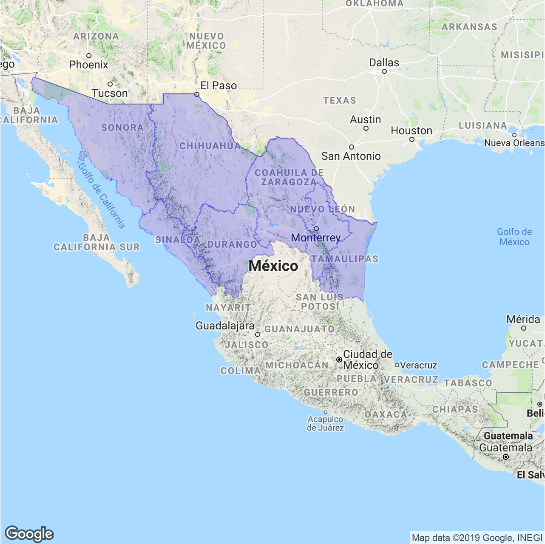
\includegraphics[width = 11cm]{ggmap_7_entidades_sample_02}  % using \graphicspath specification
\caption{Selección de 7 estados de la República Mexicana para la modelación. Este mapa fue construido con el uso de \texttt{ggmap} \citep{Kahle2013ggmap} y requirió la activación de los servicios de Google Maps.}
\label{fig:selecc_entidades_01}
\end{figure}